/home/glib/Annales/data/annales.sty
\versionAuteur

\def\changemargin#1#2{\list{}{\rightmargin#2\leftmargin#1}\item[]}
\let\endchangemargin=\endlist 
\usepackage{booktabs}
\usepackage{pdfpages}
\usepackage{listings}
\usepackage{color}
 
\definecolor{codegreen}{rgb}{0,0.6,0}
\definecolor{codegray}{rgb}{0.5,0.5,0.5}
\definecolor{codepurple}{rgb}{0.58,0,0.82}
\definecolor{backcolour}{rgb}{0.95,0.95,0.92}
 
\lstset{
    escapeinside={\\}{}, 
    basicstyle=\tiny  
    backgroundcolor=\color{backcolour},   
    commentstyle=\color{codegreen},
    keywordstyle=\color{magenta},
    numberstyle=\tiny\color{codegray},
    stringstyle=\color{codepurple},
    basicstyle=\footnotesize\ttfamily,
    breakatwhitespace=false,         
    breaklines=true,                 
    captionpos=b,                    
    keepspaces=true,                 
    numbers=left,                    
    numbersep=5pt,                  
    showspaces=false,                
    showstringspaces=false,
    showtabs=false,                  
    tabsize=2
}

\setlength{\parindent}{0cm}

\DeclareRobustCommand{\rchi}{{\mathpalette\irchi\relax}}
\newcommand{\irchi}[2]{\raisebox{\depth}{$#1\chi$}}

\usepackage{pdfpages}
\usepackage{hyperref}
\usepackage[toc,page]{appendix} 

\newcommand{\poo}{{p_{0 0}}^{-s}}
\newcommand{\pii}{{p_{1 1}}^{-s}}
\newcommand{\poodeux}{{p_{0 0}}^{-2s}}
\newcommand{\piideux}{{p_{1 1}}^{-2s}}
\newcommand{\poi}{{p_{0 1}}^{-s}}
\newcommand{\pio}{{p_{1 0}}^{-s}}
\newcommand{\poiio}{{(p_{0 1}\,p_{1 0})}^{-s}}
\newcommand{\pooii}{{(p_{0 0}\,p_{1 1})}^{-s}}




\begin{document}



% \titre{Numerical simulations of LZ78 for Markovian sources}
% Veuillez ne pas modifier ce titre SVP.
% En cas de doute, pr�venez votre coordinateur.
% Compilez par: "latex main.tex".


\separation
\bk

% Quelques explications sur le sujet; articulation des parties; une page.



%%%%%%%%%%%%%%%%%%%%%%%%%%%%%%%%%%%%%%%%%%%%%%%%%%%%%%%%%%%%%%%%%%%%%%%%%%%%%%



\medskip

\section{Conditions of the experiment}
\subsection{Simulation details}

Simulations in this report follow this experimental
process :
	
\begin{itemize}

	\item Generating a random Markov chain of size 2 of matrix
 \centers{ $\begin{matrice}
			p_{0 0} & p_{0 1} \\
			p_{1 0} & p_{1 1} \\
		  \end{matrice}$}	 
 \item
 Generating $n_{\text{exp}} \sim 10^3$ words of length $n $ (or $n_{\text{word}}$), with $n \leq 10^6 - 10^7$
 
 \item Applying LZ78 on each of these words to estimate, for each $n$,
 the number of phrases $M_n$. A simple histogram of these values
 can be seen in figure 1.
 
 \item From this sampling of the random variable $M_n$ and other parameters such as the entropy of the Markov chain, computing
 
 	\begin{itemize}
 		\item the empirical mean ($\mu$) and the empirical variance ($\sigma^2$)
 		\item different theoretical expressions of the mean and variance
 	\end{itemize}
 	
 \item Using these expressions to standardize $M_n$ in different ways, plotting
 
 	\begin{itemize}
 		\item the probability distribution of $M_n$ (standardized)
 			  
 		\item the cumulative distribution function of $M_n$ (standardized)
 	\end{itemize}
 
 \item Finally, comparing the different theoretical expressions for the mean and 
 variance by plotting their differences for a large range of values of $n$, and
 a constant number of experiments $n_{\text{exp}}$.
\end{itemize}
 
%  \subsection{Example histogram}
%  This histogram represents the counts of the different 
%  values taken by $M_n$ for $n=10^6$. 
%  Each tick on the x-axis is a data point.
 
%  \centers{
%   \begin{minipage}{7cm}
   
    		
%         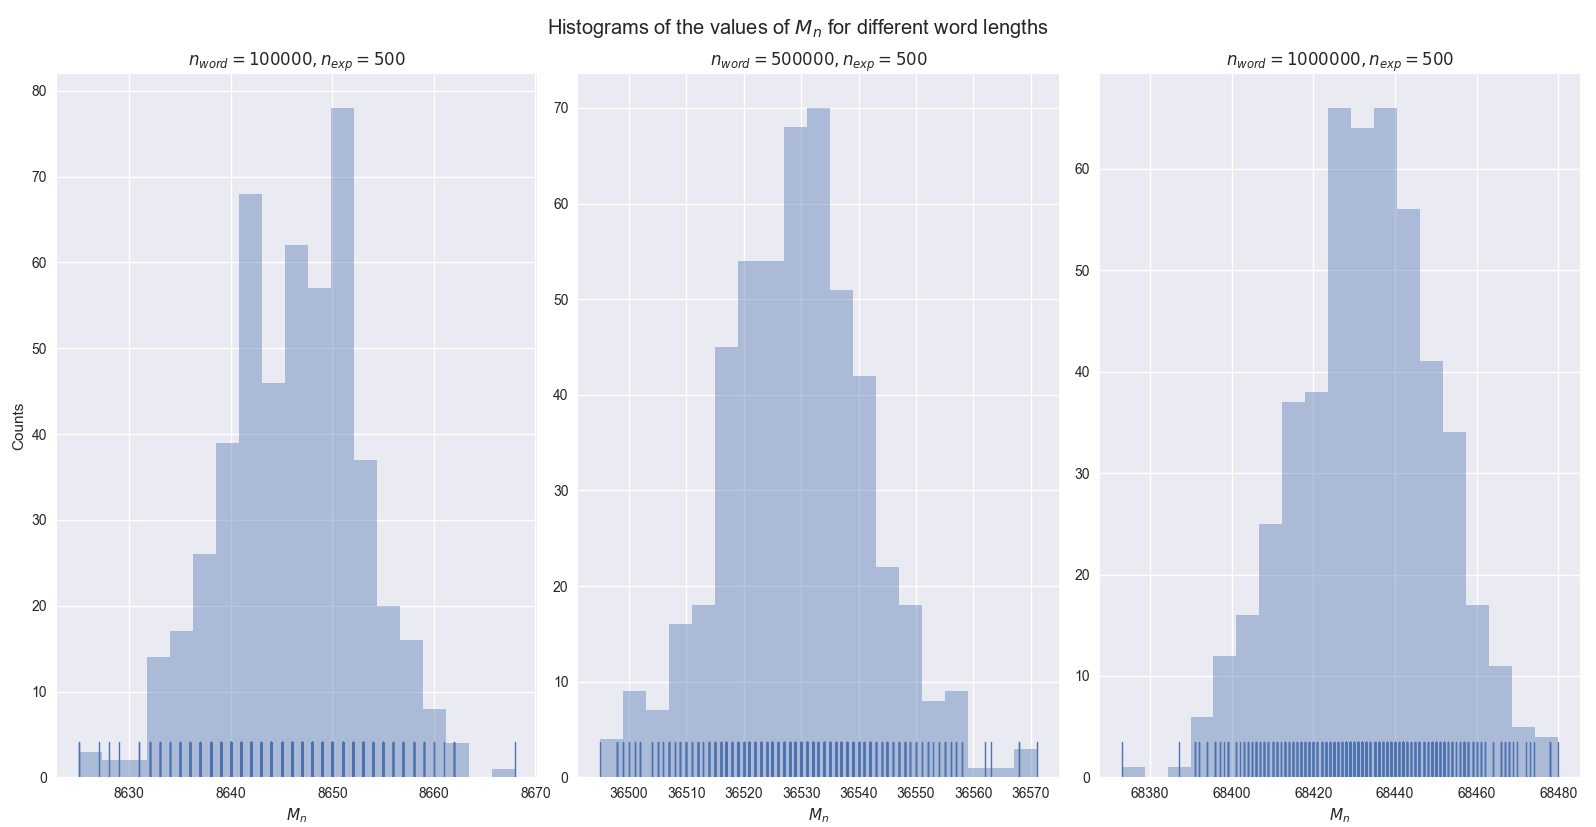
\includegraphics[width = 7cm,
%         				    trim = 27cm 0 0 0,
%         				    	clip=true]{M_n_raw_10e6_500.png}	
       
    
% 	\end{minipage}
% }

	\subsection{Empirical normalization}
 Using the empirical mean ($\mu$) and variance ($\sigma^2$) of the dataset to normalize $M_n$,
 this is a plot of the normalized distribution, compared to the normal distribution 
 in red :
 \centers{
  \begin{minipage}{6cm}
        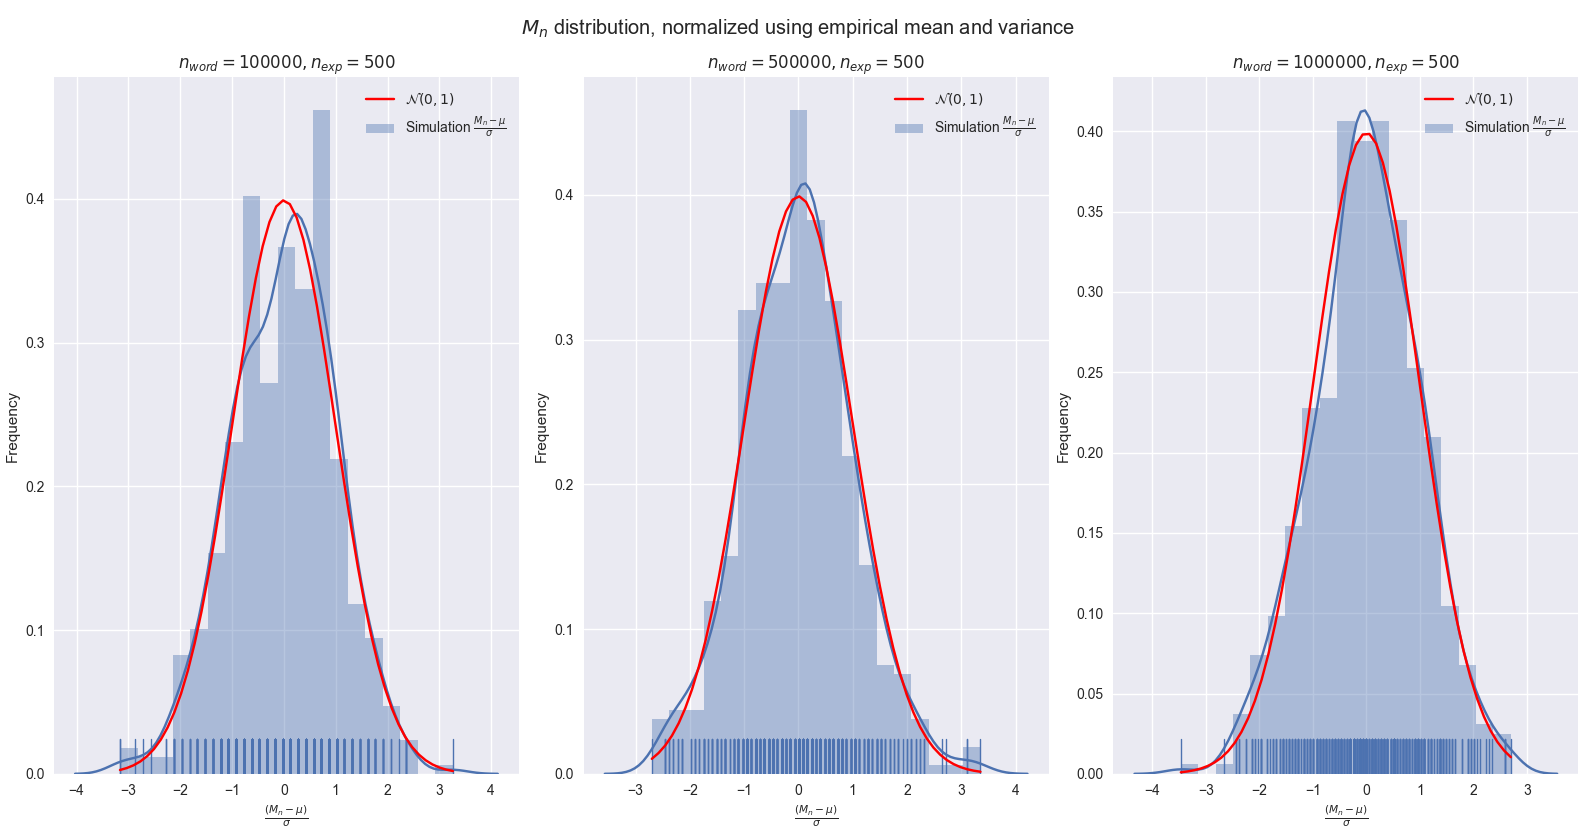
\includegraphics[width = 6cm,
        				    trim = 26.7cm 0 0 30,
        				    	clip=true]{empirical_normalization_10e6_500.png}	
	\end{minipage} 
}
	\noindent
	 and its cumulative distribution function in green, compared to the normal one in red:
 	\centers{
 	 \begin{minipage}{7cm}
        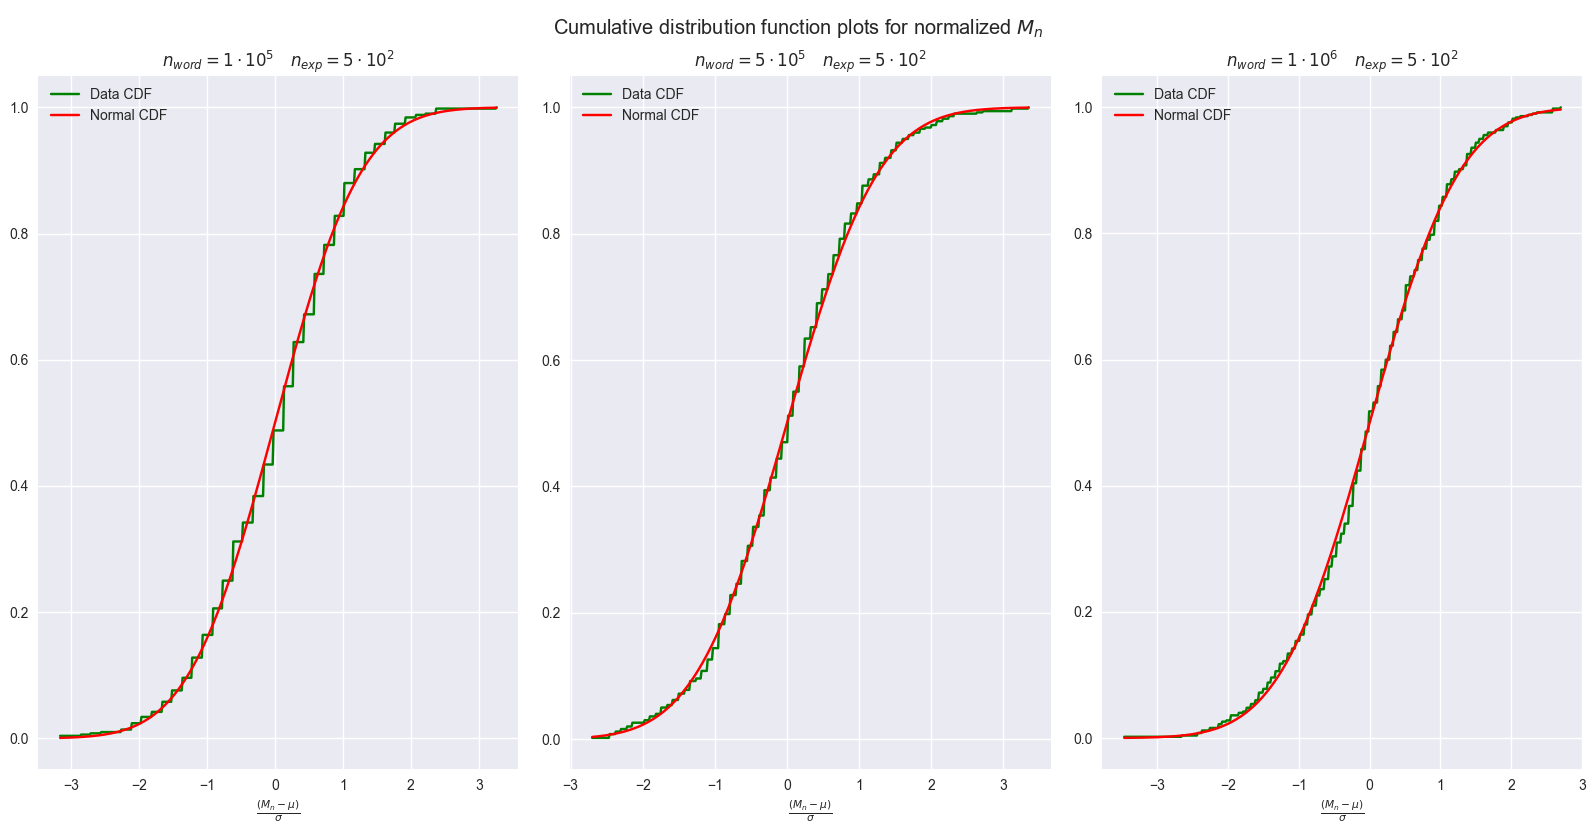
\includegraphics[width = 7cm,
        				    trim = 27cm 0 0 32,
        				    	clip=true]{cdf_1e6_500.png}
	\end{minipage} 
	}
	
	These simulations and figures strongly indicate that the general distribution
	of $M_n$ respects the central limit theorem. We now experiment with
	candidates for the variance of $M_n$ : $V_n$

	% In comments, because not really interesting
	% \centers{\question{Theoretical mean}}
	% I also tried to normalize $M_n$ using theoretical expressions
	% of the mean and variance. For the mean, the first order expression
	
	% \centers{$E_n \sim \f{nh}{\log_2(n)}$}
	
	% \noindent
	% is, under $n\leq 10^6$, not sufficient to center the distribution. I conducted a numerical analysis
	% of the difference between this expression and the empirical mean for growing 
	% values of $n$. In particular, here is how their difference, in black, compares with
	% different approximation functions 
	
	% \centers{
 	%  \begin{minipage}{9cm}
    %     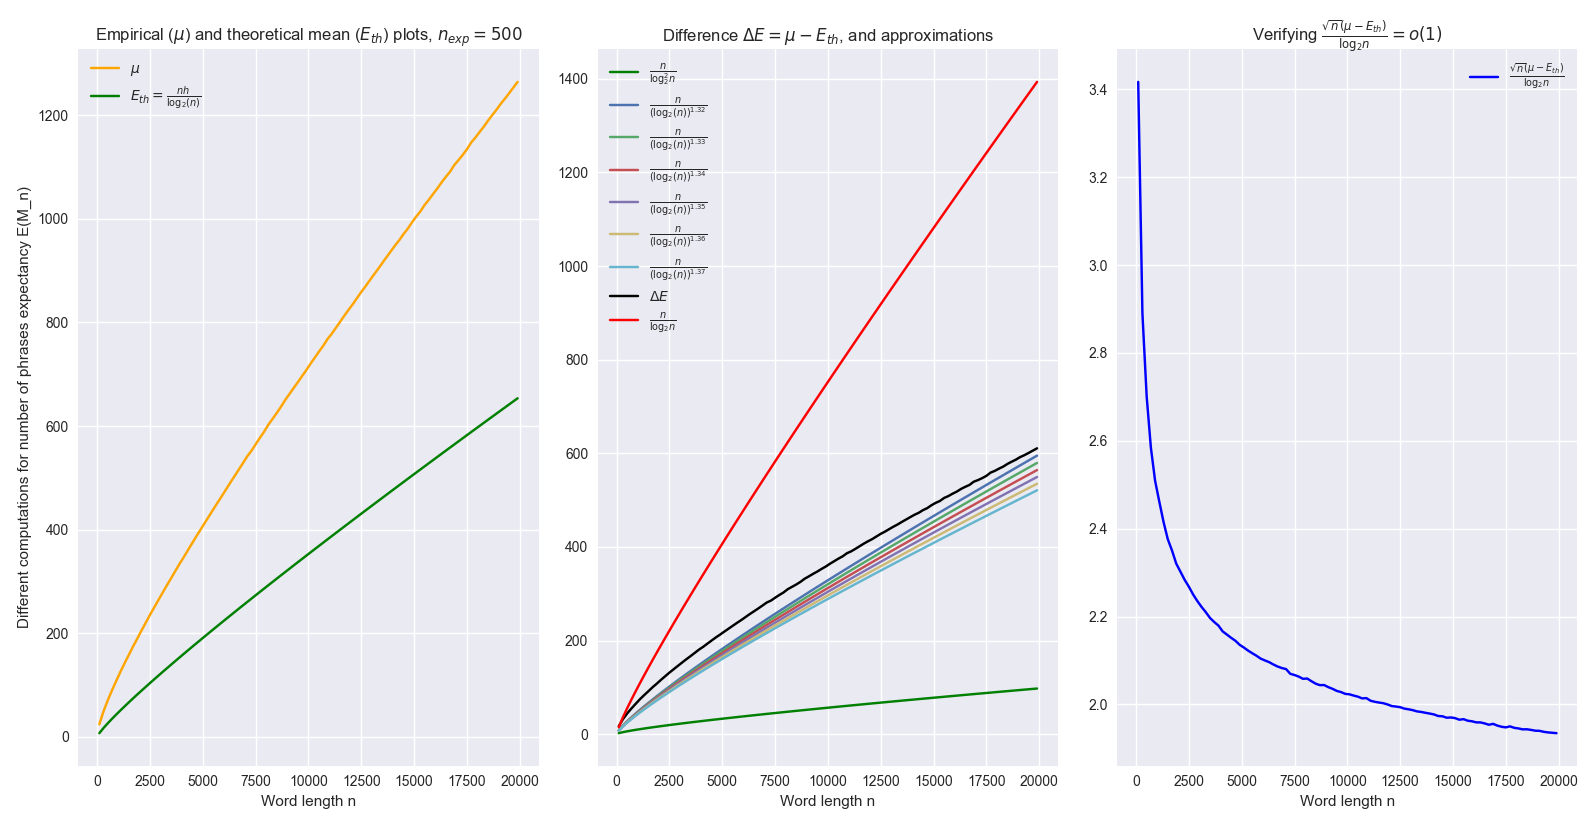
\includegraphics[width = 9cm,
    %     				    trim = 14cm 0 13cm 20,
    %     				    	clip=true]{mean_analysis_2e4_500.png}	
	% \end{minipage} 
	% }
	
	% \noindent
	% This is not troubling as it was already predicted in the formula:
	
	% \centers{$E_n = 	\f{nh}{\log_2(n)} + \mathcal{O} \pa{ \f{n}{\log_2(n)} }$}
	
	% \pagebreak
	\section{Validating variance candidates}
	\subsection{A first expression}
	As it will be used in the next section, this is the detail of the expression

		\centers{ $\f{H^3 \sigma^2}{n \log_2^2 (n)}$ }
		
	from K. Lecket, N. Wormald and R. Neininger's paper 
	\textit{Probabilistic Analysis of Lempel-Ziv Parsing for Markov Sources},  :
		
	\centers{$\sigma^2 = \sigma_0^2 + \sigma_1^2$}
	\leftcenters{where}{$\sigma_i^2 = \f{\pi_i p_{i 0} p_{i 1}}{ H^3 } \pa { \log_2 \pa{ \f{ p_{i 0} }{ p_{i 1} } }
										+ \f{H_1 - H_0}{p_{0 1} + p_{1 0}} }^2$}
	\leftcenters{with}{$\pi_0 = \f{p_{1 0}}{p_{1 0} + p_{0 1}} \qquad \pi_1 = \f{p_{0 1}}{p_{1 0} + p_{0 1}}$}
	\leftcenters{and}{$H_i = -p_{i 0} \log_2(p_{i 0}) - p_{i 1} \log_2(p_{i 1}) \qquad H = \pi_0 H_0 + \pi_1 H_1 $}
	
	% \begin{remarque}
	% \noindent 
	% The first term in the squared part of $\sigma_i^2$ accounts for the expression of the variance for memoryless sources:
	
	% \begin{egalites}
	% & \ p_{i 0}\,p_{i 1} \log_2^2 \pa{ \f{p_{i 0} }{ p_{i 1} }}
	% 	& p_{i 0} \log_2^2(p_{i 0}) + p_{i 1} \log_2^2(p_{i 1}) 
	% 		- (- p_{i 0} \log_2(p_{i 0})  - p_{i 1} \log_2(p_{i 1}))^2 \\
	% 	&& h_2 - h^2
	% \end{egalites}
	
	% \end{remarque}	
	
	% \noindent
	% It seems, from simulations, that this variance is too small and doesn't
	% catch up with the empirical variance. Here is how they compare when plotted
	% together :
	
	% \centers{
 	%  \begin{minipage}{11cm}
    %     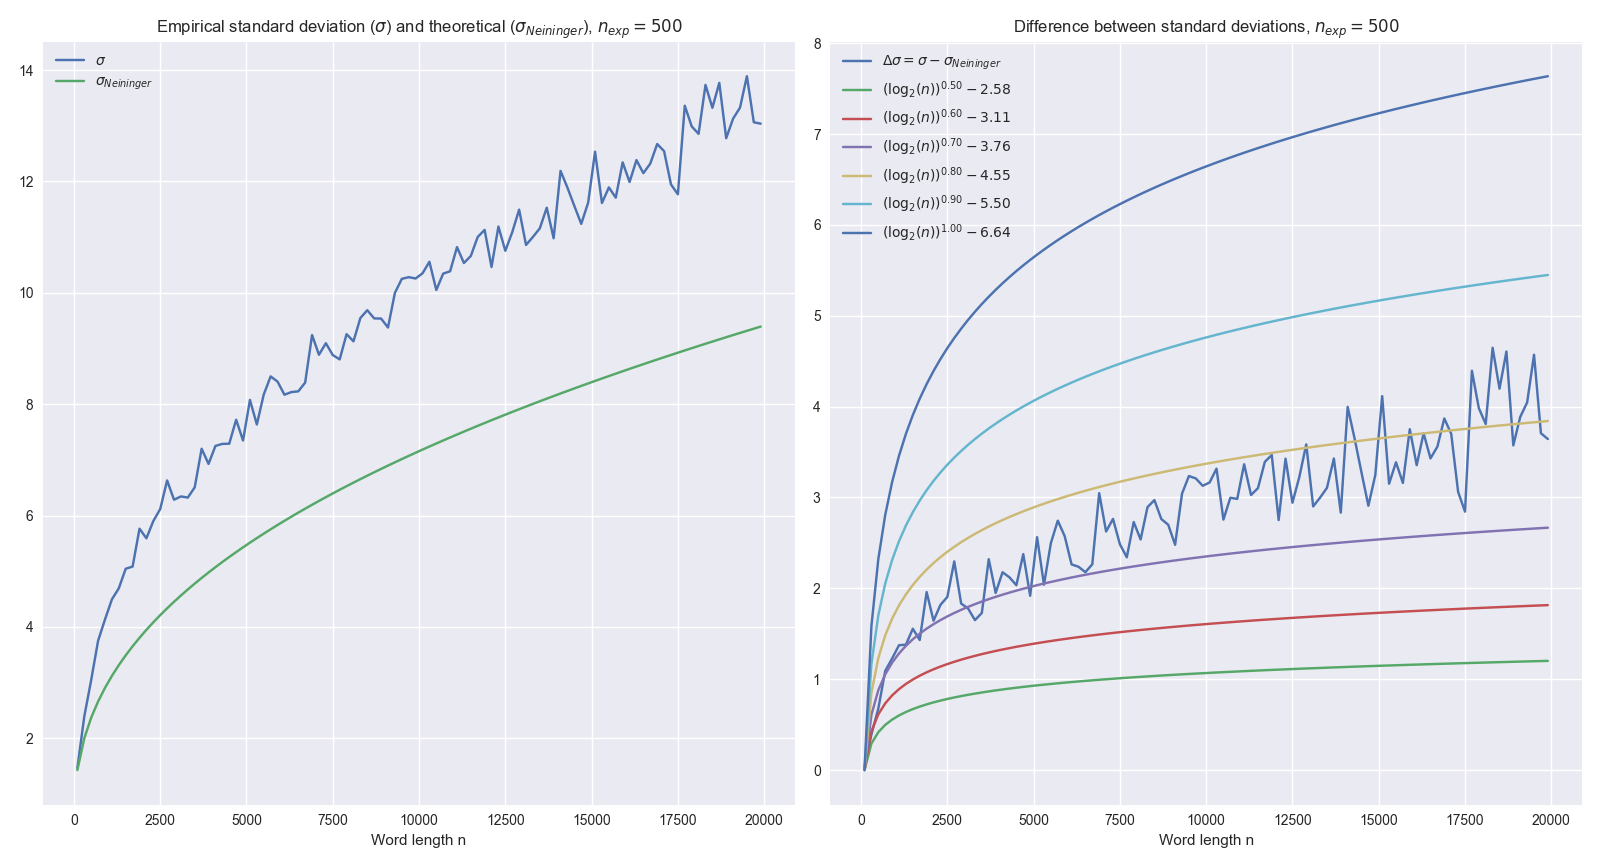
\includegraphics[width = 11cm,
    %     				    trim = 15 0 20cm 0,
    %     				    	clip=true]{std_analysis_2e4_500.png}	
	% \end{minipage} 
	% }
	
	% \pagebreak
	% \noindent
	% It seems, at first glance, that the increase would asymptotically be 
	% simply logarithmic
	
	% \centers{
 	%  \begin{minipage}{12cm}
    %     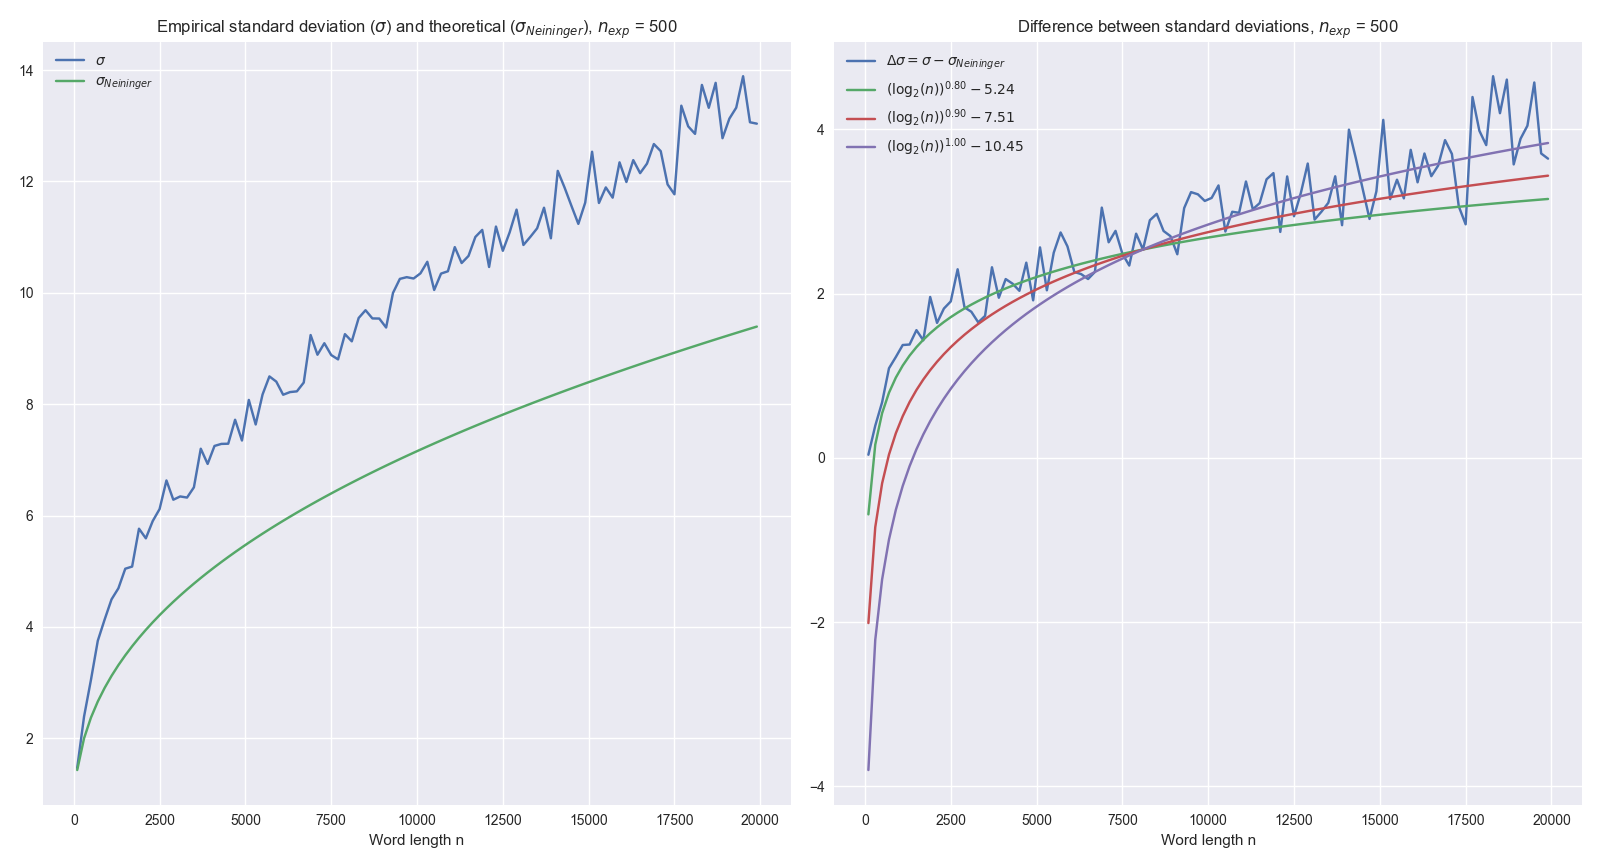
\includegraphics[width = 12cm,
    %     				    trim = 20.5cm 0 0 0,
    %     				    	clip=true]{std_analysis_approx_2e4_500.png}	
	% \end{minipage} 
	% }
	
	% \noindent 
	
	
% Now, I'm trying to compute the variance using the formula from	Jacquet and Szpankowski, 
	\textit{Average profile of the Lempel-Ziv parsing scheme for a markovian source},
	using the formula for the variance $V_n$ :
	
	\centers{$V_n = \f{1}{h^3} \pa{
                -\f{\beta}{\omega} 
                -\f2{\omega} \pi \dot{Q}^{\star} \psi 
                -h^2 } \log(m) $}
	
This formula is obtained in the Markov independent model, so
$m$ is the number of sequences with which
we build a DST. Therefore, in my case, I would take

\centers{$ m \sim \f{n h}{\log(n)} $}

I computed the other terms from the general case as follows : 

	\begin{egalites}
	Since 
		& Q(s) & \begin{matrice}
							1 - {p_{0 0}}^{-s} & -{p_{0 1}}^{-s}  \\
							-{p_{1 1}}^{-s} & 1 - {p_{1 1}}^{-s}  \\
						  \end{matrice} \\[5mm]
	then
		& Q'(s) & \begin{matrice}
							\ln(p_{0 0}) {p_{0 0}}^{-s} & \ln(p_{0 1}) {p_{0 1}}^{-s}  \\
							\ln(p_{1 0}) {p_{1 1}}^{-s} & \ln(p_{1 1}) {p_{1 1}}^{-s}  \\
						  \end{matrice} \\[5mm]
	and
		& Q''(s) & \begin{matrice}
							-\ln^2(p_{0 0}) {p_{0 0}}^{-s} & -\ln^2(p_{0 1}) {p_{0 1}}^{-s}  \\
							-\ln^2(p_{1 0}) {p_{1 1}}^{-s} & -\ln^2(p_{1 1}) {p_{1 1}}^{-s}  \\
						  \end{matrice} \\[5mm]
	hence 
		& \det Q''(s)
			&  {(p_{0 0}\, p_{1 1})}^{-s} \ln^2 p_{0 0} \cdot \ln^2 p_{1 1}
				- {(p_{0 1}\, p_{1 0})}^{-s} \ln^2 p_{0 1} \cdot \ln^2 p_{1 0} \\
	\end{egalites}

	\leftencadre
		{therefore}
		{$ \beta = \rest{\pac{\det Q''(s)}}{s=-1} = p_{0 0}\, p_{1 1} \ln^2 p_{0 0} \cdot \ln^2 p_{1 1}
				- p_{0 1}\, p_{1 0} \ln^2 p_{0 1} \cdot \ln^2 p_{1 0} $}

	\begin{egalites}
	After that, with
		& {Q^\star}(s) & \begin{matrice}
							1 - {p_{1 1}}^{-s} & {p_{0 1}}^{-s}  \\
							{p_{1 0}}^{-s} & 1 - {p_{0 0}}^{-s}  \\
						  \end{matrice} \\[5mm]
	which gives
		& {\dot{Q}^\star}(s) & \begin{matrice}
							\ln(p_{1 1}) {p_{1 1}}^{-s} & - \ln(p_{0 1}) {p_{0 1}}^{-s}  \\
							- \ln(p_{1 0}) {p_{1 0}}^{-s} & \ln(p_{0 0}) {p_{0 0}}^{-s}  \\
						  \end{matrice}
	\end{egalites}

	\leftencadre
		{then}
		{$ \pi \dot{Q}^{\star} \psi =
			\pi_0 \, p_{1 1} \, \ln (p_{1 1}) 
			- \pi_1 \, p_{1 0} \ln (p_{1 0})
			- \pi_0\, p_{0 1} \ln (p_{0 1}) \\
			 	  + \pi_1 \, p_{0 0} \ln (p_{0 0})$}

	Finally since $Q^\star = \omega \Pi$
with $\Pi = \begin{matrice} \pi_0 & \pi_1 \\
							\pi_0 & \pi_1 
			\end{matrice}$, then in particular 
			
	\centers{$1 - p_{0 0} = q_{0 0}^\star = \omega \pi_0 = \omega \f{ p_{1 0}}{p_{1 0} + p_{0 1}}$}

    \leftencadre
		{so}
		{$ \omega = \f{ (p_{0 1} + p_{1 0}) \, (1 - p_{1 1})}
						  { p_{1 0} } = p_{0 1} + p_{1 0} $}


\begin{tabular}{lrrrrrrrr}
\toprule
{} &  2o/pqpsi &         V\_n &  beta/omega &       h\textasciicircum2 &  h\textasciicircum3 values &      logs &    omegas &        unhs \\
\midrule
0 &           -0.096184 &   17.562029 &   -0.623749 &  0.220193 &    0.103325 &  3.631080 &  0.802159 &    9.678203 \\
1 &            0.489107 &    4.683284 &   -0.868024 &  0.234073 &    0.113247 &  3.661644 &  0.434225 &    8.830250 \\
2 &           -0.496605 &  747.846171 &   -0.388158 &  0.019911 &    0.002810 &  2.429464 &  0.831697 &  355.926183 \\
3 &            0.001069 &    0.926064 &   -0.501488 &  0.433778 &    0.285694 &  3.970094 &  0.997360 &    3.500248 \\
4 &            0.934518 &   -6.943693 &   -0.965841 &  0.167062 &    0.068283 &  3.493010 &  0.294606 &   14.644827 \\
5 &           -0.039947 &    3.287372 &   -0.434456 &  0.319125 &    0.180277 &  3.816619 &  1.407304 &    5.547010 \\
6 &            0.044734 &   -0.079016 &   -0.513799 &  0.475516 &    0.327905 &  4.016028 &  0.931207 &    3.049666 \\
7 &            0.088811 &   -0.104380 &   -0.547647 &  0.467153 &    0.319292 &  4.007156 &  0.871306 &    3.131927 \\
8 &            0.169804 &    1.038286 &   -0.474413 &  0.266313 &    0.137432 &  3.726165 &  1.250839 &    7.276301 \\
9 &           -0.253274 &   68.726370 &   -0.569139 &  0.105030 &    0.034039 &  3.260952 &  0.837022 &   29.378420 \\
\bottomrule
\end{tabular}




\subsection{Using the Frobenius eigenvalue of $P(s)$}

\noindent
An expression which seems to be succesful for the variance is :

\centers{$ V_n =  \left( \ddot{\lambda}(-1) - { \dot{\lambda}(-1) }^2 \right) \f{n}{\ln^2 n} $}

\noindent Let's compute $\ddot{\lambda}(-1)$ with a Markov chain of order 1.

\leftcenters
    {In the paper,}
    {$ \ddot{\lambda}(-1) = \pi \ddot{P}(-1)\psi
                        + 2 \dot{\pi}(-1) \dot{P}(-1) \psi
                        - 2 \dot{\lambda}(-1) \dot{\pi}(-1) \psi $}
\noindent However, the relations defining $\pi(s)$ : 
   
        \centers{ $ \left\{
            \begin{array}{rl} \pi(s) P(s)  &= \lambda(s) \pi(s) \\
                          P(s) \psi(s) &= \lambda(s) \psi(s) \\
                          \pi(s) \psi(s) &= \lambda(s) 
            \end{array}
                    \right. $}
         
did not seem to allow me to directly compute $\dot{\pi}(s)$ (it seemed like I need
one more).
Therefore, I computed $\lambda(s)$ as the greatest 
eigenvalue of $P(s)$. Let $\chi$ the characteristic polynomial of $P(s)$,
and $\Delta$ its discrimant

\centers{$ \chi = (X - {p_{0 0}}^{-s}) 
                  (X - {p_{1 1}}^{-s}) 
                    - (p_{0 1} \, p_{1 0})^{-s} $}

\begin{egalites}
 and   & \Delta 
        & (\poo + \pii)^2 - 4[\pooii - \poiio] \\[2mm]
        && {p_{0 0}}^{-2s} 
                + {p_{1 1}}^{-s} - 2\pooii + 4\poiio
\end{egalites}

 Informally, we have this expression for $\lambda(s)$ 
where we need to decide which sign is the correct one :
\encadre{$ \lambda(s) = \f{ \poo + \pii \pm \sqrt{\Delta(s)}}{2} $}

\leftcenters
    {Since}
    {$\Delta(-1) 
        = (p_{0 0} + p_{1 1})^2 
                        - 2 p_{0 0} p_{1 1} 
                        + 4 p_{0 1} p_{1 0}
        = (p_{0 0} + p_{1 1} - 2)^2 $}
then $ \sqrt{ \Delta(-1) } = 2 - p_{0 0} - p_{1 1} = p_{0 1} + p_{1 0}$. 
Thus, picking the $+$ sign in the former expression, we verify that  
\centers{$ \lambda(-1) =  \f{ p_{0 0} + p_{1 1} + \sqrt{ \Delta(-1) } }
                                               {2} = 1 $}

\leftcenters
    {Derivating}
    {$ \dot{\lambda}(s) = \f12 \left( -\ln p_{0 0}\, \poo - \ln p_{1 1}\, \pii + \f{ \Delta'(s) }{ 2 \sqrt{\Delta(s)} } \right) $}

and the expression for $\Delta'(s)$
\centers{$ \Delta'(s) = - 2 \ln p_{0 0}\, \poodeux - 2 \ln p_{1 1}\, \piideux
                        + 2 \ln (p_{0 0} p_{1 1})\, \pooii 
                        - 4 \ln (p_{0 1} p_{1 0})\, \poiio $}
gives
\centers{$ \Delta'(-1) = - 2 \ln p_{0 0}\, {p_{0 0}}^2 - 2 \ln p_{1 1}\, {p_{1 1}}^2
                        + 2 \ln (p_{0 0} p_{1 1})\, (p_{0 0} p_{1 1})
                        - 4 \ln (p_{0 1} p_{1 0})\, (p_{0 1} p_{1 0})  $}

allowing to compute $\dot{\lambda}(-1)$. 
Numerically, we verified that $ \dot{\lambda}(-1) = h $. Derivating again yields

\centers{$ \ddot{\lambda}(s) =
                \f12 \left( \ln^2 p_{0 0} \poo + \ln^2 p_{1 1} \pii
                    + \f{ \Delta''(s) \sqrt{\Delta(s)} - \Delta'(s) \cdot \tf{\Delta'(s)}
                                                                            {2\sqrt{\Delta(s)}} }
                        {2\Delta(s)} \right)
                   $}

\leftcenters
    {with}
    {$ \Delta''(s) = 4 \ln^2 p_{0 0}\, \poodeux + 4 \ln^2 p_{1 1}\, \piideux
                     - 2 \ln^2 (p_{0 0} p_{1 1})\, \pooii
                     + 4 \ln^2 (p_{0 1} p_{1 0})\, \poiio $}

\leftencadre
    {Finally}
    {$\ddot{\lambda}(-1) = \f12 \left( \ln^2 p_{0 0}\, p_{0 0} + \ln^2 p_{1 1}\, p_{1 1}
                                + \f{ \Delta''(-1) \sqrt{\Delta(-1)} - \tf { {\Delta'(-1)}^2 }
                                                                              {2\sqrt{\Delta(-1)}} }
                                        {2\Delta(-1)} \right)
                         $}

The simulations using this coefficient for the variance are quite good. It also seems that 
this formula for the variance is equivalent to the one used in the unpublished paper 
\emph{Probabilistic Analysis of Lempel-Ziv Parsing for Markov Sources} by Leckey, 
Wormald and Neininger, but our two ways of deriving it differs. Numerical instability
might account for the tiny differences found for high $n$ values ($10^7$), although
this hasn't been verified. 
The code that computes it can be found in appendix \ref{app:comp_lam2},
and the rest of the code, with detailed procedures for reproducibility,
is hosted on GitHub in a repository that, for the moment, private.
Another way of computing $\lambda(s)$ is in appendix \ref{app:comp_lam1}. 

\centers{
 	 \begin{minipage}{11cm}
        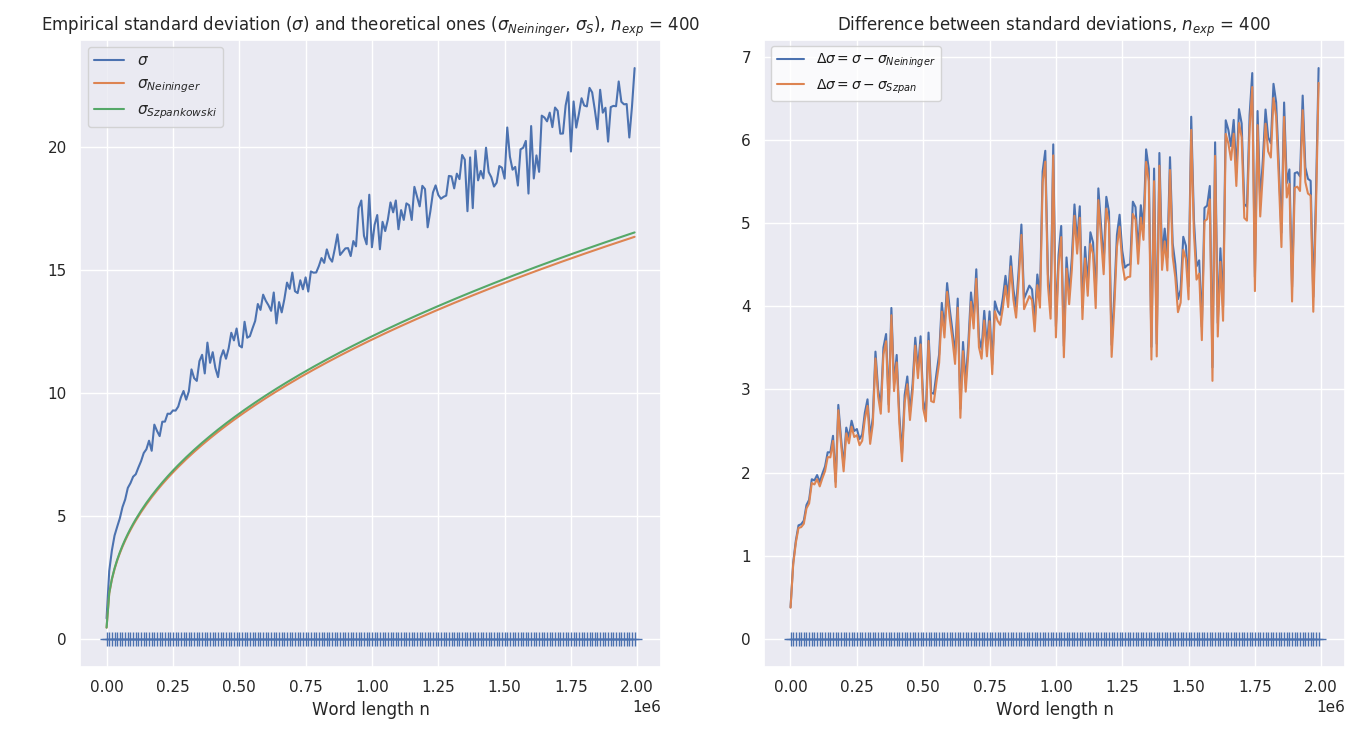
\includegraphics[width = 11cm,
        				    trim = 0 0 16.5cm 0,
        				    	clip=true]{./figs/eig_fig1.png}	
	\end{minipage} 
	}

\centers{
 	 \begin{minipage}{11cm}
        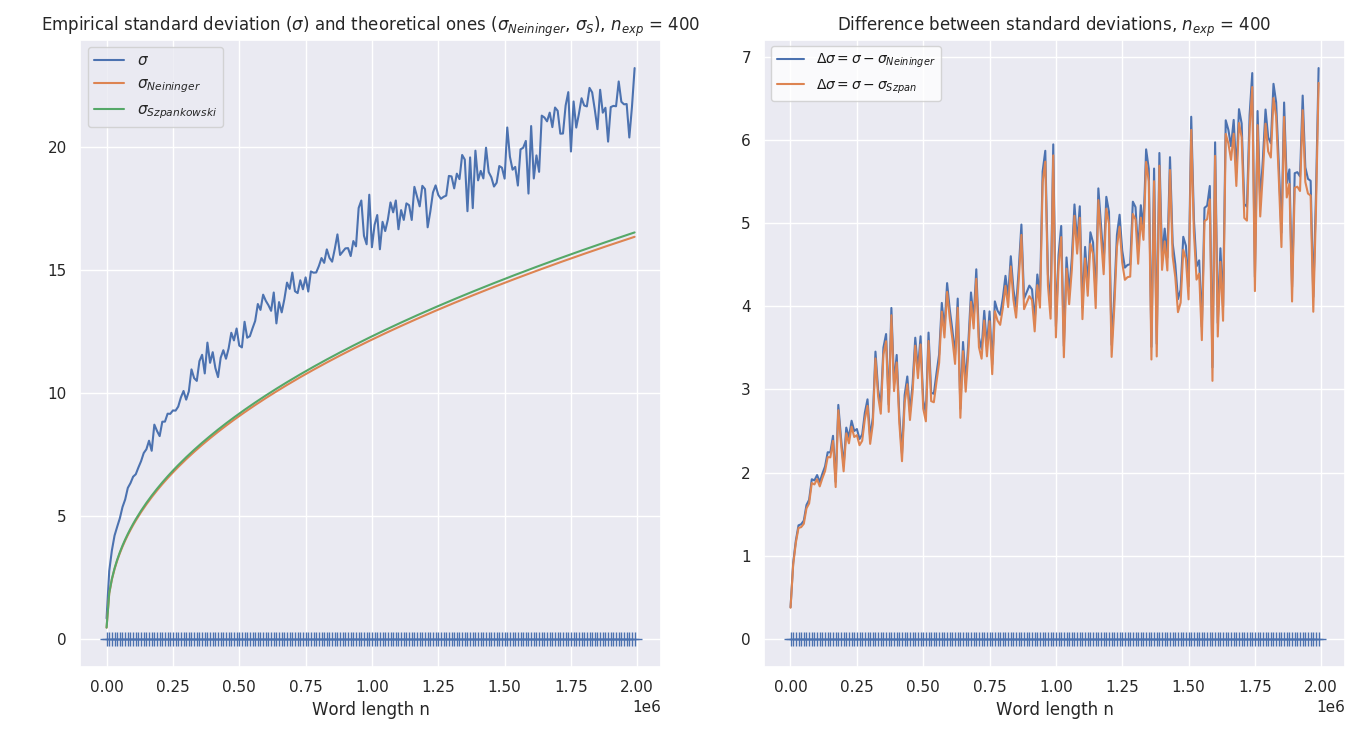
\includegraphics[width = 11cm,
        				    trim = 18.5cm 0 0 0,
        				    	clip=true]{./figs/eig_fig1.png}	
	\end{minipage} 
	}

\pagebreak
Now, for some distributions of very long words that were normalized using 
our theoretical standard deviations, and empirical means. The blue plot is 
a gaussian fit for the simulation results, which also appear as a blue histogram.
The two sets of figures are identical but obtained using different expressions.

\noindent
 	 \begin{minipage}{\textwidth}
        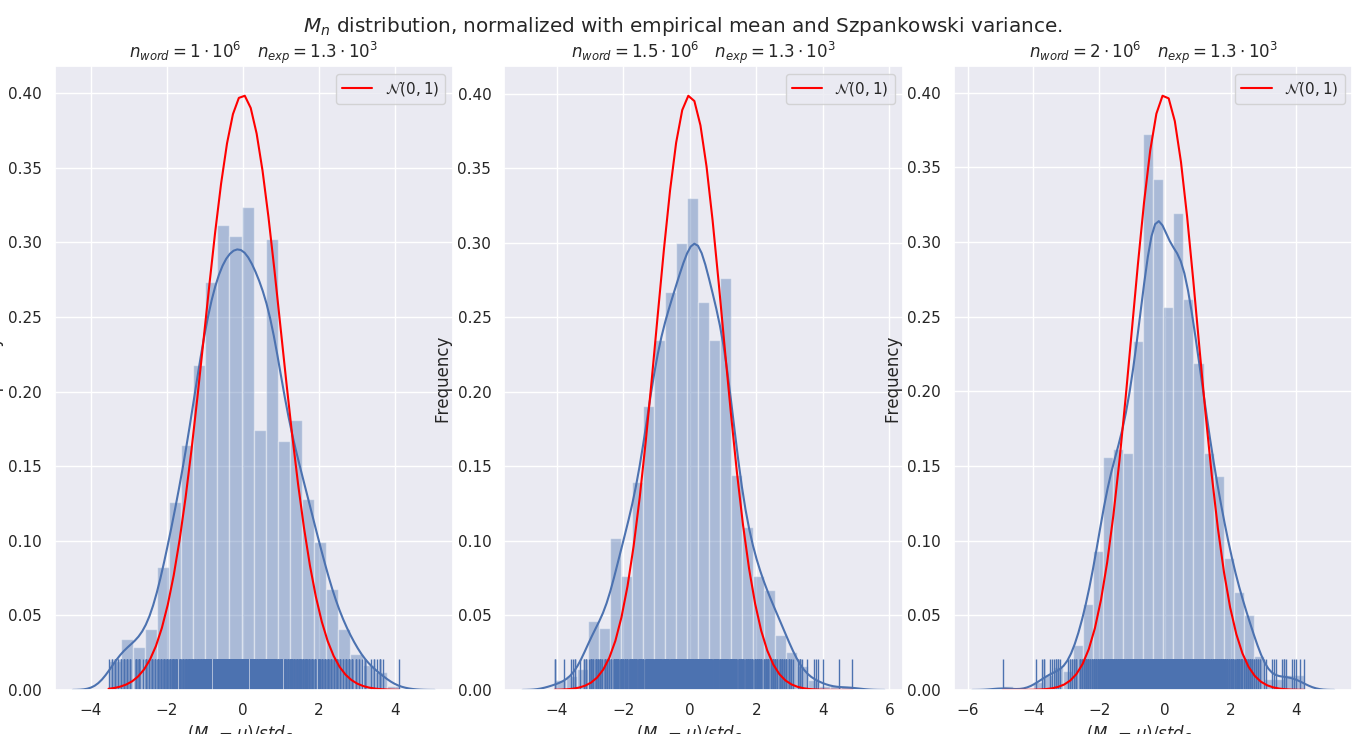
\includegraphics[width = \textwidth,
        				    trim = 0 0.5cm 0 0,
        				    	clip=true]{./figs/eig_fig2.png}	
	\end{minipage} 

\noindent
 	 \begin{minipage}{\textwidth}
        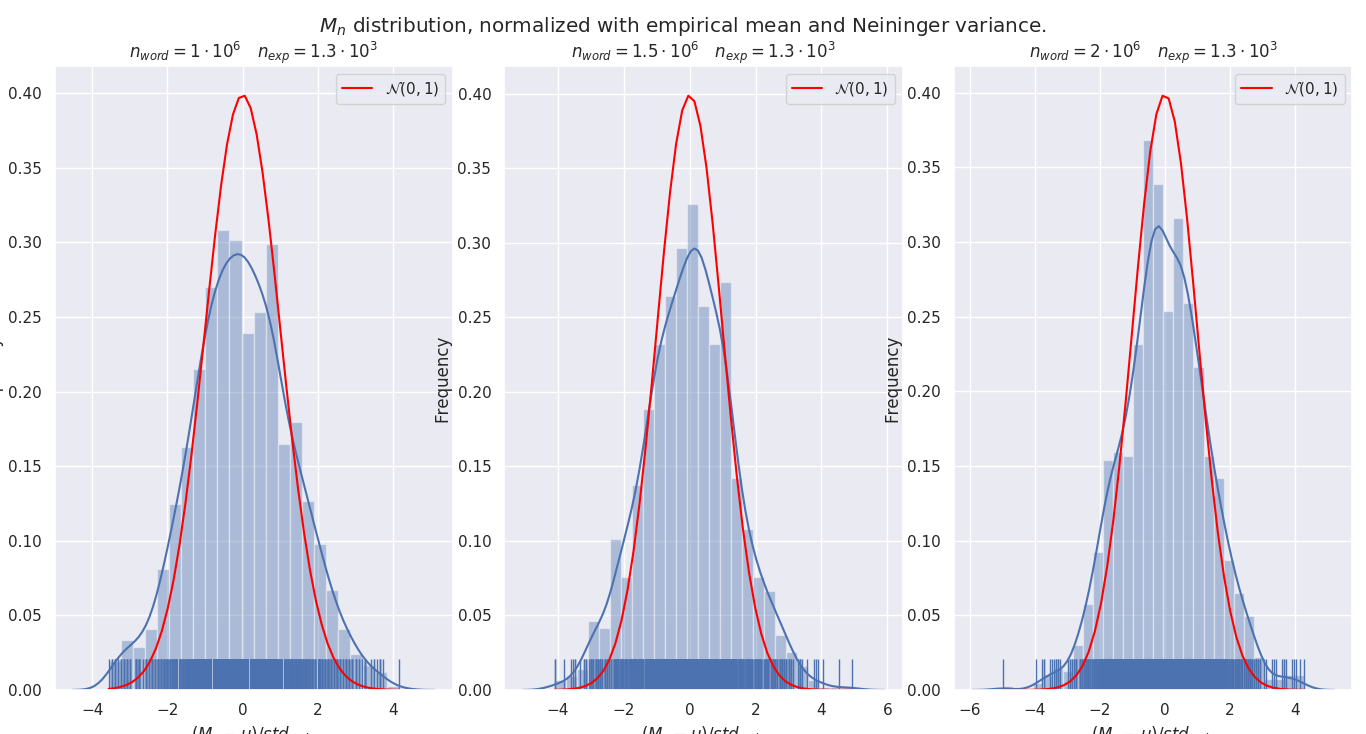
\includegraphics[width = \textwidth,
        				    trim = 0 0.5cm 0 0,
        				    	clip=true]{./figs/eig_fig3.png}	
	\end{minipage} 


\section{Conclusion}
Similar results were obtained for a variety of randomly generated Markov sources,
which seem to indicate that this formula for the variance could be proven theoretically
correct. 

\begin{remarque}
\noindent \textbf{Limits of this work}


The figures suffer from imprecision over the computation of the empirical 
variance : this is due to the difficulties encountered in computing large amounts
of long words (of size over $10^6$). The figure in appendix \ref{app:much_longer} is 
an example of this limitation : with only 100 experiments, the empirical variance 
varies a lot. Possible ideas of improvement might come from parallelization,
rewriting functions in a computationnal language such as Julia, or using/devising a datastructure
specific to the task of building very long words.

Another problem is that the space of random Markov chains (here: stochastic matrices
of size 2) is not sampled thoroughly, therefore this claim might only seem to hold for some
specific Markov chains. Sampling a small number of Markov chains uniformly
according to their entropy might be interesting as a representation of the space,
 because otherwise it would be hard to sample a large number of stochastic matrices
due to the necessity of computing large words for each of them.

Finally, the difference between empirical $V_n$ and our expression seems to be growing
very slowly with $n$. This might be a term that is negligible (\textit{i.e.} of 
order lower than $\tf{n}{\log_2^2(n)}$), or a small detail in the formula of $V_n$. 
For example, the natural base logarithm (in $\tf{n}{\ln^2(n)}$) in the eigenvalue expression works slightly
better than the one in base 2 (in $\tf{n}{\log_2^2(n)}$), with the inverse situation happening for the first 
expression ($\sigma_{\text{Neininger}}$). Anyway, the figures obtained seem to 
indicate that we are close to the exact solution.

\end{remarque}



 
% \noindent First term is
% \centers
%     { $\pi_0 \, p_{0 0} \, \log^2 (p_{0 0}) 
%         + \pi_1 \, p_{1 0} \, \log^2 (p_{1 0}) 
%         + \pi_0 \, p_{0 1} \, \log^2 (p_{0 1}) 
%         + \pi_1 \, p_{1 1} \, \log^2 (p_{1 1})  $}

% \noindent The second is
% \centers
%     { $ - 2 \pac{
%             \dot{\pi}_0(-1) p_{0 0} \log (p_{0 0})    
%             + \dot{\pi}_1(-1) p_{1 0} \log (p_{1 0}) 
%             + \dot{\pi}_0(-1) p_{0 1} \log (p_{0 1})
%             + \dot{\pi}_1(-1) p_{1 1} \log (p_{1 1})
%         }   
%     $}

% \noindent The third is
% \centers{
%     $ - 2 \dot{\lambda}(-1) \pac{
%         \dot{\pi}_0(-1) 
%         + \dot{\pi}_1(-1)
%     }$
% }

% \noindent We 
%         have to compute $\dot{\pi}(-1)$. With 
%             $\pi(s) = (\pi_0(s), \, \pi_1(s))$, and since

% \centers{$\pi(s) P(s) = \lambda(s) \pi(s)$}

% \leftcenters
%     {then we have}
%     {$ \left\{
%         \begin{aligned}
%             {p_{0 0}}^{-s} \pi_0(s) + {p_{0 1}}^{-s} \pi_1(s) &= \lambda(s) \pi_0(s) \\
%             {p_{1 0}}^{-s} \pi_0(s) + {p_{1 1}}^{-s} \pi_1(s) &= \lambda(s) \pi_1(s) \\
%         \end{aligned}
%         \right.
%      $}

% which I'm not sure how to solve formally.
% \noindent
% solving for $\pi_0(s)$ and $\pi_1(s)$, 
% assuming $ p_{0 0} p_{1 1} \neq p_{0 1} p_{1 0} $ :

% \centers{$ \pi_0(s) = \lambda(s) \f{ \overbrace{{p_{1 1}}^{-s} - {p_{0 1}}^{-s}}^{g_0(s)} }
%                                    { \underbrace{{ (p_{0 0} p_{1 1}) }^{-s} 
%                                         - { (p_{0 1} p_{1 0}) }^{-s}}_{\delta(s)} }
%             \qquad 
%             \text{and}
%             \qquad
%        \pi_1(s) = \lambda(s) \f{ \overbrace{{p_{0 0}}^{-s} - {p_{1 0}}^{-s}}^{g_1(s)} }
%                                    { { (p_{0 0} p_{1 1}) }^{-s} 
%                                         - { (p_{0 1} p_{1 0}) }^{-s} }$}


% \leftcenters
%     {hence for $i\in\{0,1\}$}
%     {$ \dot{\pi}_i(s) = \dot{\lambda}(s) \f{g_i(s)}{\delta(s)}
%                         + \lambda(s) \f{{g_i}'(s)\delta(s) - g_i(s)\delta'(s)}
%                                         {\delta^2(s)}$}

% \leftcenters
%     {so}
%     {$ \dot{\pi}_i(-1) = h \f{g_i(-1)}{\delta(-1)}
%                         + \f{{g_i}'(-1) \delta(-1) - g_i(-1) \delta'(-1) }
%                             {\delta^2(-1)} $}

% \begin{egalites}
%     with & \delta(-1) 
%             & p_{0 0} p_{1 1} - p_{0 1} p_{1 0} \\[3mm]
%          &g_0(-1) 
%             & p_{1 1} - p_{0 1} \\[3mm]
%         &{g_0}'(-1)
%             & -\ln (p_{1 1}) p_{1 1} + \ln (p_{0 1}) p_{0 1} \\[3mm]
%         &g_1(-1)
%             & p_{0 0} - p_{1 0} \\[3mm]
%         &{g_1}'(-1) 
%             & -\ln (p_{0 0}) p_{0 0} + \ln (p_{1 0}) p_{1 0} 
% \end{egalites}


% \leftcenters
%     {where}
%     {  $\left\{
%         \begin{minipage}{0.6\textwidth}
%        $ {g_0}'(s) = - \ln(p_{1 1}) {p_{1 1}}^{-s}
%                  + \ln(p_{0 1}) {p_{0 1}}^{-s}$ \\[3mm]
%         $\delta'(s) = - \ln( p_{0 0} p_{1 1}) { (p_{0 0} p_{1 1}) }^{-s}
%                         +  \ln ( p_{0 1} p_{1 0} ) { (p_{0 1} p_{1 0}) }^{-s} $
%         \end{minipage}
%         \right.$ }



% \noindent
% Now taking $s=-1$ and re-arranging in a linear system of unknown $\dot{\pi}_0(-1)$ and $\dot{\pi}_1(-1)$ :
% \centers
%     {$ \left\{
%         \begin{aligned}
%             \dot{\pi}_0(-1) (p_{0 0} - \lambda)
%             + \dot{\pi}_1(-1) p_{0 1}
%                 &= \dot{\lambda}(-1) \pi_0
%                     +   \ln p_{0 0} \cdot p_{0 0} \pi_0
%                     +   \ln p_{0 1} \cdot p_{0 1} \pi_1 \\
%             \dot{\pi}_0(-1) p_{1 0}
%             + \dot{\pi}_1(-1) (p_{1 1} - \lambda)
%                 &= \dot{\lambda}(-1) \pi_1
%                     +  \ln p_{1 0} \cdot p_{1 0} \pi_0 
%                     +  \ln p_{1 1} \cdot p_{1 1} \pi_1
%         \end{aligned}
%         \right.
%      $}

% \noindent since
% $\dot{\lambda}(-1) = h$ and,
% $\lambda(-1) = 1$ :

% \centers
%     {$ \left\{
%         \begin{aligned}
%             \dot{\pi}_0(-1) (p_{0 0} - 1)
%             + \dot{\pi}_1(-1) p_{0 1}
%                 &= h \pi_0
%                     +   \ln p_{0 0} \cdot p_{0 0} \pi_0
%                     +   \ln p_{0 1} \cdot p_{0 1} \pi_1 \\
%             \dot{\pi}_0(-1) p_{1 0}
%             + \dot{\pi}_1(-1) (p_{1 1} - 1)
%                 &= h \pi_1
%                     +  \ln p_{1 0} \cdot p_{1 0} \pi_0 
%                     +  \ln p_{1 1} \cdot p_{1 1} \pi_1
%         \end{aligned}
%         \right.
%      $}

% \begin{egalites}
% which is  &\lambda
%         &\f{ (p_{0 0} + p_{1 1}) 
%            + \sqrt{ (p_{0 0} + p_{1 1})^2 - 4 (p_{0 0} p_{1 1} - p_{1 0} p_{0 1}) }}
%            {2}\\[3mm]
%         &&\f{ (p_{0 0} + p_{1 1}) 
%            + \sqrt{ (p_{0 0} - p_{1 1})^2 + 4 p_{1 0} p_{0 1} }}
%            {2}   
% \end{egalites}







\begin{thebibliography}{9}

    \bibitem{avg}
        \textsc{Jacquet}, \textsc{Szpankowski}, \textsc{Tang},
        \textit{Average profile of the Lempel-Ziv parsing scheme for a Markovian source}

\end{thebibliography}

\end{document}
